\chapter{Appendices for Chapter \ref{ch:Stannigel2012}}
\label{app:Stannigel2012}


\section{Phonon nonlinearities}

In Eq. (8) in the main text we have derived an effective master equation (ME) to
describe the nonlinear interaction between two phonon modes. In the following we
present an alternative, more rigorous, approach, which illustrates the
individual approximations made in the derivation of the effective phonon
nonlinearity in more detail. We first consider only a single mechanical mode,
e.g. $b\equiv b_1$, which also allows us more easily to compare the results with
exact numerical calculations of the full model.


\subsection{Model}

We start with the full ME for the two optical modes coupled to a single
resonator mode, which in the frame of the driving frequency $\omega_L$ can be
written as
\begin{equation}\label{eq:SM_ME}
\dot \rho = -i[H_0+H_g+ H_\Omega(t),\rho] + \mathcal{L}_{\rm diss} \rho. \\
\end{equation}
Here 
\begin{equation}
H_0=  \omega_m b^\dag b - \Delta_s c_s^\dag c_s - \Delta_a  c_a^\dag c_a, 
\end{equation}
and
\begin{equation}
H_g= \frac{g_0}{2} \left(c_a c_s^\dag b^\dag +    c_a^\dag c_s  b \right),
\end{equation}
are the free evolution and the OM coupling, respectively,  $H_\Omega(t)=
i\Omega_s(t) (c_s^\dag - c_s)$ is the driving field for the symmetric mode with
slowly varying amplitude $\Omega_s(t)$ and
\begin{equation}
\mathcal{L}_{\rm diss} \rho  = \sum_{\eta=s,a} \kappa \mathcal{D}[c_\eta] \rho +
\frac{\gamma}{2} \mathcal{D}_{\rm th}[b]  \rho,
\end{equation}
accounts for dissipation. Here we have defined the superoperator
$\mathcal{D}_{\rm th}[b] = (N_{\rm th}+1)  \mathcal{D}[b] +  N_{\rm th} 
\mathcal{D}[b^\dag]$ to describe the coupling to a thermal bath.



\subsection{Displaced frame}

In contrast to the approach outlined in the main text, we now start our analysis
with a unitary displacement $U(t) c_sU^\dag (t)= c_s +\alpha(t)$ where the
classical cavity field $\alpha(t)$ obeys
\begin{equation}
\dot \alpha(t)= (i\Delta_s - \kappa) \alpha(t)  + \Omega_s(t). 
\end{equation}�
This unitary transformation eliminates the classical driving field and in the
new frame the resulting ME can be written as
\begin{equation}\label{eq:SM_FullME}
\begin{split}
\dot \rho = &-i[H_{\rm lin}+H_g,\rho] + \mathcal{L}_{\rm diss} \rho, \\
\end{split} 
\end{equation}
where $H_\Omega(t)$ has disappeared, but the linear part of the Hamiltonian now
contains an additional coupling between the resonator and the anti-symmetric
cavity mode,
\begin{equation}\label{eq:Hlin}
H_{\rm lin}�=  H_0  + G(t) c_a b^\dag + G^*(t) c_a^\dag b,
\end{equation} 
where $G(t)=g_0 \alpha(t)/2$. Note that ME \eqref{eq:SM_FullME} is still exact
and we will use this equation for our exact numerics below.


\subsection{Hybridized modes}

To proceed, we assume that $\alpha(t)$ is constant or slowly varying on the
timescale set by the detunings $|\Delta_a+\omega_m^i|$. This allows us to write
$H_{\rm lin}$ in its adiabatic eigenbasis
\begin{equation}
H_{\rm lin}�= - \Delta_s c_s^\dag c_s  - \tilde \Delta_a C^\dag C + \tilde
\omega_m B^\dag B,
\end{equation}
where  the $C$ and $B$ are bosonic operators for the hybridized mechanical and
optical modes and $\tilde \Delta_a$ and $\tilde \omega_m$ are the new
eigenfrequencies of $H_{\rm lin}$ for a given $G\equiv G(t)$.   We obtain
\begin{eqnarray}
C&=& \cos(\theta) c_a - \sin(\theta) b,\\
B&=& \cos(\theta) b + \sin(\theta) c_a,
\end{eqnarray}
where $\tan(2\theta)=-2|G|/\delta$ and
$\delta=-(\Delta_a+\omega_m)=2J-\omega_m-\Delta_s$. The shifted frequencies are
given by
\begin{eqnarray}
-\tilde \Delta_a&=& -\Delta_a - \frac{1}{2}\left( \delta - \sqrt{\delta^2+4|G|^2
}\right),\\
\tilde \omega_m &=& \omega_m - \frac{1}{2}\left( \delta +\sqrt{\delta^2+4|G|^2
}\right).
\end{eqnarray}
We see that by slowly increasing the classical control field $\alpha(t)$, the
mechanical mode $b$ is adiabatically converted into a polaronic mode $B$. For
small mixing angles $\theta$ the mode still retains its mechanical character,
while the finite photonic component is responsible for inducing an effective
nonlinearity.

In terms of the hybridized mode operators the dissipative terms can be written
as
\begin{equation}\label{eq:SM_Ldiss}
\begin{split}
\mathcal{L}_{\rm diss}\simeq& \kappa \mathcal{D}[c_s] + \kappa \cos^2(\theta)
\mathcal{D}[C] +   \frac{\gamma}{2}�\sin^2(\theta) \mathcal{D}_{\rm th}[C]  \\
+&  \frac{\gamma}{2}�\cos^2(\theta) \mathcal{D}_{\rm th}[B] + \kappa
\sin^2(\theta) \mathcal{D}[B]�.
\end{split} 
\end{equation}
In particular, we identify an additional optical decay channel with rate
$\gamma'=2 \kappa \sin^2(\theta)$ for the $B$ mode. In the following we define 
as
\begin{equation}
\tilde{\mathcal{L}}_\gamma =   \frac{\gamma}{2}�\cos^2(\theta)
\mathcal{D}_{\rm th}[B] + \frac{\gamma^\prime}{2} \mathcal{D}[B],
\end{equation}
the modified mechanical dissipation Liouvillian.
Note that in Eq.~\eqref{eq:SM_Ldiss} we have already neglected cross-terms
between $C$  and $B^\dag$. This is valid in the parameter regime considered
below, where $\kappa$ is small compared to the splitting of these two modes.
 

Finally, we also express the nonlinear interaction $H_g$ in terms of the
hybridized modes and write the result as
\begin{equation}\label{eq:SM_HgDecomp}
H_g= H_g^{(1)} + H_g^{(2)} + H_g^\prime. 
\end{equation}
Here, the first term is the one of interest 
\begin{equation}
H_g^{(1)} = \frac{g_0}{4}  \sin(2\theta)  \left( c_s + c_s^\dag\right) B^\dag B
,
\end{equation}
and describes the coupling of the $c_s$ mode to the number operator of the $B$
mode.
The second term is given by
\begin{equation}
H_g^{(2)} = -\frac{g_0}{2}  \sin^2(\theta)  \left( B  c_s^\dag C^\dag  + B^\dag 
c_s C \right),
\end{equation}
and leads to additional corrections. However, for small $\theta$ this term is
small compared to $H_g^{(1)}$. It can be further reduced if 
$|\Delta_s-\delta|\gg \Delta_s$.
Finally, the last term contains interactions
\begin{equation}
H_g^{\prime} = \frac{g_0}{2}  \cos^2(\theta)  \left( C c_s^\dag B^\dag  +
C^\dag  c_s B \right)  - \frac{g_0}{4}  \sin(2\theta)  \left( c_s +
c_s^\dag\right) C^\dag C,
\end{equation}
which can be neglected when either the $c_s$ or the $C$ mode are in the vacuum
state.


\subsection{Adiabatic elimination of the cavity mode}

Our goal is now to derive an effective ME for the mechanical degrees of freedom
only. To do so, we write the full ME as
\begin{equation}
\dot \rho = \left(\mathcal{L}_0 + \mathcal{L}_1\right)\rho,
\end{equation}
where 
\begin{equation}
\mathcal{L}_0\rho = -i[H_{\rm lin}+ H_g^\prime,\rho] + \mathcal{L}_{\rm diss}
\rho,
\end{equation}
and
\begin{equation}
\mathcal{L}_1\rho = -i[H_{g}^{(1)}+ H_g^{(2)},\rho].
\end{equation}
The dynamics of $\mathcal{L}_0$ does not excite the cavity modes, and therefore,
in the limit where $\tilde g=g_0\sin(2\theta)/4\rightarrow 0$ (either $g_0$ is
small or the mixing angle $\theta$ is small) the density operator can to a good
approximation be written as $\rho(t)=\rho_m(t) \otimes \rho_c^0$, where
$\rho_c^0$ is the vacuum state of the $c_s$ and the $C$ mode. To account for the
effects of a small $\mathcal{L}_1\sim\tilde g$ up to second order in
perturbation theory we define a projection operator onto this subspace,
\begin{equation}
\mathcal{P}\rho = {\rm Tr}_c\{ \rho \}\otimes \rho_c^0,
\end{equation}
and its complement $\mathcal{Q}=\mathds{1}-\mathcal{P}$. Then
\begin{eqnarray}
\mathcal{P}\dot \rho&=& \mathcal{P}\mathcal{L}_0\mathcal{P} \rho + \mathcal{P}
\mathcal{L}_{1}\mathcal{Q}\rho,\\
\mathcal{Q}\dot \rho&=& \mathcal{Q}(\mathcal{L}_0+\mathcal{L}_{1})\mathcal{Q}
\rho +  \mathcal{Q}\mathcal{L}_{1}\mathcal{P}\rho.
\end{eqnarray}
 Up to second order in $\tilde g$ we can formally integrate the equation for
 $\mathcal{Q}\rho$ and obtain
\begin{equation}
\mathcal{P}\dot{\rho}(t)\simeq\mathcal{P}\mathcal{L}_{0}\mathcal{P}\rho(t)+\mathcal{P}\mathcal{L}_{1}\int_{0}^{\infty}
 d\tau\, \mathcal{Q}
e^{\mathcal{L}_{0}\tau}\mathcal{Q}\mathcal{L}_{1}\mathcal{P}\rho(t).
\end{equation}
We define by $\rho_m(t)={\rm Tr}_c\{\mathcal{P} \rho(t)\}$ the reduced density
operator of the mechanical mode and write the final result as
\begin{equation}\label{eq:SM_Lm}
\dot\rho_m(t)=\left( \mathcal{L}^{(0)}_m+  \mathcal{L}^{(1)}_m   + 
\mathcal{L}^{(2)}_m\right) \rho_m(t).
\end{equation}
The first term describes the linear part of the dynamics  
\begin{equation}
\mathcal{L}^{(0)}_m \rho_m=  -i[ \tilde \omega_m B^\dag B,\rho_m] + 
\tilde{\mathcal{L}}_\gamma \rho_m,
\end{equation} 
with a modified frequency and modified decay rates for the $B$ mode. The other
two terms are given by
\begin{equation}\label{eq:SM_Lm1}
\mathcal{L}^{(1)}_m \rho_m = - \int_{0}^{\infty}  d\tau\, {\rm Tr}_c\{
[H_{g}^{(1)} , e^{\mathcal{L}_{0}\tau}\left([H_{g}^{(1)},\rho_m \otimes 
\rho_c^0] \right) ]\},
\end{equation}
and
\begin{equation}\label{eq:SM_Lm2}
\mathcal{L}^{(2)}_m \rho_m = - \int_{0}^{\infty}  d\tau\, {\rm Tr}_c\{
[H_{g}^{(2)} , e^{\mathcal{L}_{0}\tau}\left([H_{g}^{(2)},\rho_m \otimes 
\rho_c^0] \right) ]\}.
\end{equation}
 

\subsection{Simple perturbation theory}

In deriving Eq.~\eqref{eq:SM_Lm} we have so far only assumed that $\tilde g$ is
small compared to the typical frequency scales of the dynamics of the  $c_s$
mode. For now we will also assume that $g_0$ is small compared to $\delta$
\emph{and} $\Delta_s$. This allows us to neglect the term $H_g^\prime$ in
$\mathcal{L}_0$ and the cavity correlation functions in Eqs.~\eqref{eq:SM_Lm1}
and \eqref{eq:SM_Lm2} can be evaluated in a straight forward manner.  For the
action of $\mathcal{L}^{(1)}_m$ we obtain
\begin{equation}
\mathcal{L}^{(1)}_m \rho_m = -i  [\Lambda (B^\dag B)^2,\rho_m] + \Gamma_\phi
\mathcal{D} [B^\dag B],
\end{equation}
where $\Lambda=  {\rm Im} \{ S^{(1)}_{gg}(0) \}$,  $\Gamma_\phi=  {\rm Re}\{
S^{(1)}_{gg}(0)\}$   and
\begin{equation}
S^{(1)}_{gg} (\omega) = \tilde g^2\int_{0}^{\infty}  d\tau\, {\rm Tr}_c\{  c_s
e^{\mathcal{L}_{0}\tau} \left(c_s^\dag \rho_c^0\right)\}�e^{-i\omega \tau} .
\end{equation} 
We find $ S^{(1)}_{gg}(\omega)= \tilde g^2/(-i(\Delta_s+\omega) + \kappa)$ and
after inserting back the definition of $\tilde g$ in the limit
$|g_0\alpha/\delta| \ll 1$  we recover the expressions for $\Lambda$ and
$\Gamma_\phi$ given in Eq. (9) in the main text.
Similarly we obtain
\begin{equation}
\mathcal{L}^{(2)}_m \rho_m = -i  [ \delta \omega_m^{(2)}  B^\dag B,\rho_m] +
\frac{\gamma^{(2)}}{2} \mathcal{D} [B],
\end{equation}
where  $\delta \omega_m^{(2)}={\rm Im} \{ S^{(2)}_{gg}(\tilde \omega_m) \}$,
$\gamma^{(2)}=  {\rm Re}\{ S^{(2)}_{gg}(\tilde \omega_m)\}$   and
\begin{equation}
S^{(2)}_{gg} (\omega) = \frac{g_0^2 \sin^4(\theta)}{4}  \int_{0}^{\infty} 
d\tau\, {\rm Tr}_c\{  c_s C e^{\mathcal{L}_{0}\tau} \left(c_s^\dag C^\dag
\rho_c^0\right)\} e^{-i\omega \tau}.
\end{equation} 
The small frequency shift $\delta \omega_m^{(2)}$ can be absorbed into the
definition of $\tilde \omega_m$ and, since $\gamma^{(2)}\approx \gamma^\prime
\sin^2(\theta) g_0^2/(4\delta^2)$, for not too large mixing angles $\theta$,
$\gamma^{(2)}$ can always be neglected compared to $\gamma^\prime$. All together
the final effective phonon master equation is
\begin{equation}\label{eq:SM_EffectiveME}
\begin{split}
\dot \rho_m =& -i[\tilde \omega_m B^\dag B + \Lambda ( B^\dag B)^2 �, \rho_m ]
 + \Gamma_\phi \mathcal{D}[B^\dag B]\rho_m \\
&  + \frac{\gamma}{2}\mathcal{D}_{\rm th}[B] \rho_m  +  \frac{\gamma^\prime}{2} 
 \mathcal{D}[B]\rho_m,
\end{split} 
\end{equation}
which is the single resonator version of ME (8) given in the main text. 


\subsection{Corrections}

Let us now extend the above result to the case where $\tilde g$ is small
compared to $\Delta_s$ and $\delta$, but the bare interaction $g_0$ is not. In
this case the general expressions in Eqs.~\eqref{eq:SM_Lm1} and
\eqref{eq:SM_Lm2} still apply, but the effect of $H_g^\prime$ must be taking
into account when evaluating the correlation functions. To illustrate this, let
us assume that $g_0$ is still small compared to $\delta$. Then, by assuming that
the $C$ mode is initially in the ground state,  we obtain  approximately
\begin{equation}
H_{\rm lin} +H_g^\prime \approx - (\Delta_s- \Delta_B B^\dag B) c_s^\dag c_s,  
\end{equation}
where  the off-resonant frequency shift is 
\begin{equation}
\Delta_B= \frac{g_0^2\cos^4(\theta)}{4(\tilde \Delta_a+\tilde\omega_m
-\Delta_s))},
\end{equation}
and  can be comparable to $\Delta_s$. Therefore, we must evaluate the
correlation function for each phonon number state $|n\rangle$ separately and
write the resulting non-linear interaction as
\begin{equation}\label{eq:SM_EffectiveME_corr}
\mathcal{L}^{(1)}_m \rho_m = \sum_n n^2\left( -i  \left[\Lambda(n)
|n\rangle\langle n|�,\rho_m\right] + \Gamma_\phi(n)  \mathcal{D}
[|n\rangle\langle n| ])\right).
\end{equation}
Here $\Lambda(n)$ and $\Gamma_\phi(n)$   are the imaginary and real part of 
\begin{equation}
 S^{(1)}_{gg}(\omega=-n \Delta_B) =\frac{ n^2 \tilde g^2}{-i(\Delta_s-n\Delta_B)
 + \kappa}.
\end{equation}
We see that in this parameter regime more complicated nonlinearities can occur,
but the overall magnitude and the ratio between coherent and dephasing
interactions remains the same. In principle, this analysis can be extended to
the regime, where $g_0$ is comparable to $\delta$. However, in this case no
simple analytic expressions for $\lambda(n)$ and $\Gamma_\phi(n)$ can be derived
and need to be evaluated numerically.


\subsection{Numerical simulation} 

\begin{figure}
\centering
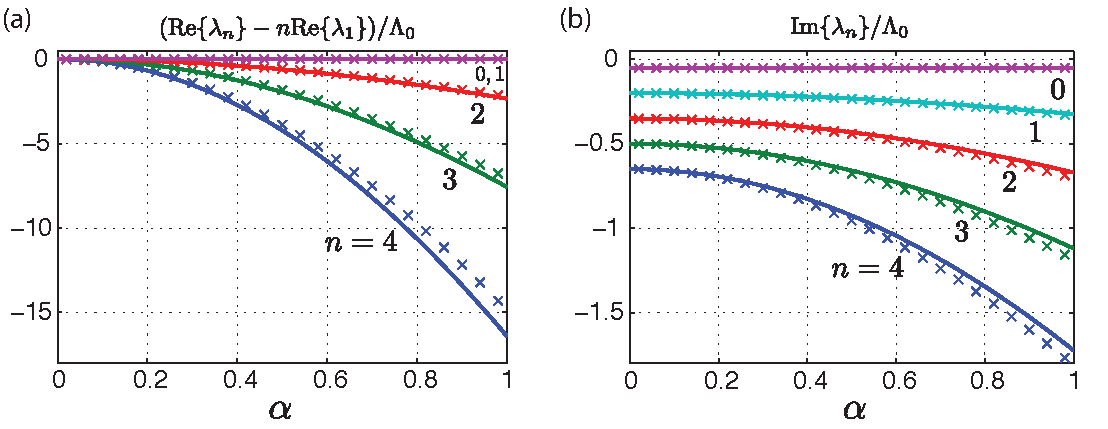
\includegraphics[width=1\textwidth]{./figs_Stannigel2012/Figure_suppl.pdf}
\caption
[Comparison of effective and exact description]
{Comparison of the effective analytic description
(Eqs.\,\eqref{eq:analytics}, lines) with exact eigenvalues of the Hamiltonian in
Eq.\,\eqref{eq:Hfull} (crosses) for different cavity field amplitudes $\alpha$.
All results are normalized to the scale
$\Lambda_0=g_0^4/(16\abs{\Delta_s}\delta^2)$ of the non-linearity.
(a) Deviation of the real parts of the eigenvalues from the result expected for
a linear oscillator, such that the splitting of the curves indicates an
effective non-linearity.
(b) Imaginary parts of the eigenvalues corresponding to decays. In both plots we
used the parameters $\Delta_s/g_0=-1$, $\delta/g_0=5$, $\kappa/g_0=2.5\times
10^{-2}$, $\gamma_m/g_0=2.5\times 10^{-4}$ and $N_{\rm th}=1$.}
\label{fig:numerics}
\end{figure}


To assess the validity of the effective phonon ME we now compare our result with
the dynamics of the full OMS.  Since we are mainly interested in the relation
between the phonon non-linearity and the corresponding dephasing and decay
rates, it is sufficient to evaluate the spectrum of the non-Hermitian
Hamiltonian, which  for the full model it is given by
\begin{equation}
\label{eq:Hfull}
\tilde H_{\rm full}=  H_{\rm lin}+ H_g - i\kappa c_s^\dag c_s - i\kappa
c_a^\dag c_a
 -i\frac{\gamma}{2} (N_{\rm th}+1) b^\dag b  -i\frac{\gamma}{2} N_{\rm th} b
b^\dag.
\end{equation}
In Fig.~\ref{fig:numerics} we plot the real and imaginary parts of the lowest
eigenvalues $\lambda_n$ of $\tilde H_{\rm full}$, which correspond to the lowest
number states $|n\rangle$ of the $B$ mode.
From the effective phonon model given in Eq.~\eqref{eq:SM_EffectiveME} and
\eqref{eq:SM_EffectiveME_corr} we obtain the approximate analytic results
\begin{subequations}
\label{eq:analytics}
\begin{equation}
{\rm Re} \{ \lambda_n\}= n \tilde \omega_m + n^2 \Lambda(n),
\end{equation}  
and
\begin{equation}
|{\rm Im} \{ \lambda_n\}|=\frac{\gamma}{2} N_{\rm th} + n \left(
\frac{\gamma}{2} (2N_{\rm th}+1) +\frac{\gamma^\prime}{2}\right) +n^2
\Gamma_\phi(n).
\end{equation}
\end{subequations}
We see a good agreement between these results for the effective model and the
exact numerics, both for the real and imaginary parts. Although there are some
deviations due to higher-order effects, the effective non-linear splitting
(Fig.~\ref{fig:numerics}(a)) is much larger than the induced decoherence
(Fig.~\ref{fig:numerics}(b)), as is expected for the chosen parameters. Hence,
we conclude that the effective model accurately describes the dynamics of the
mechanical resonator, and that the effective phonon non-linearity may serve as a
basis for gate operations as discussed in the main text and in the following
section.


\section{Phonon-phonon interactions} 

The derivation of the effective phonon nonlinearity, as outlined above for a
single resonator, can be easily adapted to two resonators as discussed in the
main text.
In this case we have 
\begin{equation}
H_0=  \sum_{i=1,2} \omega^i_m b_i^\dag b_i - \Delta_s c_s^\dag c_s - \Delta_a 
c_a^\dag c_a,
\end{equation}
and
\begin{equation}
H_g= \frac{g_0}{2} \left[c_a c_s^\dag (b^\dag_1-b_2^\dag) +    c_a^\dag c_s 
(b_1-b_2)\right].
\end{equation}
After changing into the displaced representation to eliminate the driving field
we obtain the linearized Hamiltonian
\begin{equation}
H_{\rm lin}�=  H_0  + \sqrt{2}\left( G(t)  c_a b_a^\dag + G^*(t) c_a^\dag
b_a\right),
\end{equation} 
where $b_a=(b_1-b_2)/\sqrt{2}$ and $G(t)=g_0\alpha(t)/2$.
For similar mechanical frequencies $\omega_m^1\simeq \omega_m^2=\omega_m$ the
symmetric resonator mode is decoupled and we can simply repeat the analysis from
above by identifying $b\equiv b_a$ and replacing $g_0$ by $\sqrt{2}g_0$.

For arbitrary $\omega_i$, we write the linear part of the Hamiltonian in its
diagonal form
\begin{equation}\label{eq:Hlin}
H_{\rm lin}�=  - \Delta_s c_s^\dag c_s -  \tilde \Delta_a  C^\dag C + \tilde
\omega_1 B_1^\dag B_1 + \tilde \omega_2 B_2^\dag B_2.
\end{equation} 
As in the single-resonator case the $c_s$ mode is unaffected,  but the $c_a$
mode now couples to both $b_1$ and $b_2$.  The resulting hybridized modes $C$,
$B_\pm$ depend on the choice of parameters $\omega_m^{1,2}, \Delta_a$ and $G$.
For the case of interest, i.e. for a symmetric detuning
$\omega_m^{1,2}=-\Delta_a \mp \delta$, we obtain
\begin{eqnarray}
C&=& \cos(2\Theta) c_a -  \sin(2\Theta)(B_1 + B_2)/\sqrt{2},\\
B_1&=& \cos^2(\Theta) b_1 + \sin(2\Theta) c_a/\sqrt{2} -  \sin^2(\Theta)b_2,\\
B_2&=& \cos^2(\Theta) b_2 + \sin(2\Theta) c_a/\sqrt{2} -  \sin^2(\Theta)b_1,
\end{eqnarray} 
where $\tan(2\Theta)=-\sqrt{2} |G|/\delta$. Therefore, for small $\Theta$ the
modes $B_{1,2}$ correspond to the original mechanical resonator modes $b_{1,2}$
and $\tilde \omega_i\approx \omega_m^{i}$.

As above, we can now re-express the dissipation and the non-linear coupling
$H_g$ in terms of $C$ and $B_\pm$. The modified mechanical dissipation terms are
given
\begin{equation}
\tilde{\mathcal{L}}_\gamma =  \sum_{i=1,2}  \frac{\gamma}{2}�\cos^2(2\Theta)
\mathcal{D}_{\rm th}[B_i] + \frac{\kappa}{2} \sin^2(2\Theta) \mathcal{D}[B_i],
\end{equation}
and for small $\Theta$ the optical decay rate $\gamma^\prime =\kappa
\sin^2(2\Theta)$ is the same as given above and in the main text.
Using the decomposition of the non-linear coupling as done in
Eq.~\eqref{eq:SM_HgDecomp},  we obtain
\begin{equation}
H_g^{(1)}= \frac{g_0}{\sqrt{8} }\sin(2\Theta)   \left( c_s+c_s^\dag\right)
\left(B_1^\dag B_1 - B^\dag_2 B_2\right),
\end{equation} 
the contribution $H_g^{(2)}$ vanishes and 
\begin{equation}
H_g^{\prime}= \frac{g_0}{2  }\cos(2\Theta)   \left( C c_s^\dag
(B_1^\dag-B_2^\dag) + {\rm H.c.}  \right).
\end{equation}
We see that the structure and also the relative frequency scales are identical
to the corresponding terms discussed for the single resonator above. Therefore,
under the same conditions we can eliminate the cavity mode and  obtain the
effective phonon master equation
\begin{equation}
\begin{split}
\dot \rho_m =& -i\left[\sum_i \tilde \omega_i B_i^\dag B_i + \Lambda (B_1^\dag
B_1-B_2^\dag B_2)^2 �, \rho_m \right]  \\
&+ \Gamma_\phi \mathcal{D}[(B_1^\dag B_1-B_2^\dag B_2)]\rho_m   +
\tilde{\mathcal{L}}_\gamma \rho_m.
\end{split} 
\end{equation}
 For small $\Theta$ this equation reduces to ME  (8) in the main text and
 higher-order corrections can be included in the same way as discussed for the
 single resonator case.
